\documentclass[11pt]{article}

\usepackage[margin=1in]{geometry}
\usepackage{graphicx}
\usepackage{booktabs}
\usepackage{amsmath}
\usepackage{xcolor}
\usepackage{hyperref}
\usepackage{enumitem}
\usepackage{caption}
\usepackage{float}

\hypersetup{colorlinks=true, linkcolor=black, citecolor=black, urlcolor=blue}

\setlength{\parskip}{0.5em}
\setlength{\parindent}{0pt}

\title{\vspace{-1.5em}Temporal Super-Sampling: Technical Report}
\author{Shiven Bajpai}
\date{}

\begin{document}
\maketitle
\vspace{-2.5em}

\section{Overview}
This report documents the technical implementation of a temporal super-sampling network that upscales rendered game frames by a factor of 2$\times$ (540p $\rightarrow$ 1080p), using auxiliary channels provided by the game engine (depth, motion vectors, and sub-pixel jitter offsets) in addition to color. The network follows a single-frame recurrent design in the style of Mercier et al.\cite{mercier2023}, in which a per-pixel blend mask combines a freshly synthesized high-resolution candidate frame with a motion-warped version of the previous output. The model is trained on a subset of the Qualcomm Rasterized Images (QRISP) dataset \cite{qrisp}.

\section{Dataset}

\subsection{Source and modalities}
A subset of the QRISP dataset (specifically the \texttt{ScifiBase} scenes) is used, containing paired low-resolution (540p, $960\times540$) and native high-resolution (1080p, $1920\times1080$) renders of the same sequences, along with auxiliary buffers rendered at the low resolution:

\begin{itemize}[itemsep=2pt]
    \item \textbf{LR color}: jittered, mip-biased color buffer (\texttt{MipBiasMinus1Jittered}).
    \item \textbf{LR depth}: packed into an 8-bit RGBA PNG and unpacked in software into a single-channel float depth map via a base-255 weighted sum of the four channels.
    \item \textbf{LR motion vectors}: stored as an EXR buffer (\texttt{MotionVectorsMipBiasMinus1Jittered}).
    \item \textbf{Per-frame camera jitter}: sub-pixel $(x,y)$ jitter offset read from a per-frame JSON camera-data file.
    \item \textbf{HR target}: native-resolution ground-truth color (\texttt{Native}).
\end{itemize}

\subsection{Preprocessing}
A preprocesser converts each scene's per-frame PNG/EXR/JSON files into contiguous, memory-mapped float32 arrays (\texttt{lr\_color.dat}, \texttt{depth.dat}, \texttt{motion.dat}, \texttt{jitter.dat}, \texttt{hr\_color.dat}) on disk, one set of files per scene, to allow fast random access during training without repeated image decoding.

\subsection{Splits and sampling}
Scenes are split 70/15/15 into train/validation/test sets at the scene level. To reduce memory footprint of individual training samples, each scene is cropped as: 
\begin{itemize}[itemsep=2pt]
    \item a \textbf{temporal} crop of consecutive frames from the scene (14 frames for training, 7 for validation), and
    \item a \textbf{spatial} crop of the low-resolution frame (only applied on training set), with the matching $2\times$ crop applied to the high-resolution target.
\end{itemize}

\section{Network Architecture}

The architecture used is a direct implementation of the model described by Mercier et. al\cite{mercier2023}. Refer to the paper for more details.

\subsection{Model configuration used}
\begin{table}[H]
\centering
\begin{tabular}{ll}
\toprule
Hyperparameter & Value \\
\midrule
Recurrent feature channels & 10 \\
Hidden feature channels & 48 \\
Convolution blocks in backbone & 3 \\
Jitter-MLP hidden width & 512 \\
Motion-vector dilation block size & 6 \\
\bottomrule
\end{tabular}
\end{table}

\section{Training Setup}

\subsection{Loss}
Training minimizes a composite objective over each predicted frame batch:
\[
\mathcal{L} = \mathcal{L}_{1} + 0.1\cdot\mathcal{L}_{\text{LPIPS(AlexNet)}} + 0.2\cdot\left(1 - \text{SSIM}\right),
\]
using the standard L1 loss, the \texttt{lpips} package's AlexNet-based perceptual metric, and the \texttt{pytorch\_msssim} SSIM implementation. A Charbonnier loss class and a hand-written SSIM function are also defined in the codebase but are not the loss used by the training loop.

\subsection{Optimization}
\begin{itemize}[itemsep=2pt]
    \item Optimizer: Adam, learning rate $2\times10^{-4}$.
    \item Scheduler: \texttt{StepLR}, step size 10 epochs, decay factor 0.5.
    \item Gradient norm clipping at 1.0.
    \item Batch size: 7 sequences; trained for 100 epochs.
    \item Sequences are processed in chunks of 7 frames to bound memory use; the recurrent state is detached and carried across chunks within a sequence, and trailing chunks shorter than 5 frames are dropped.
\end{itemize}

\subsection{Metrics and validation}
PSNR (computed as $10\log_{10}(1/\text{MSE})$ on the $[0,1]$-normalized color output) and the training loss are logged every epoch on the training set. A full validation pass runs every 10 epochs, logging validation loss/PSNR and exporting a qualitative debug image comparing bicubic-upsampled input, prediction, ground truth, and absolute error for the first validation batch.

\subsection{Environment}
The notebook was run on Google Colab (T4 GPU). 

\section{Results}

\subsection{Training curves}
\begin{figure}[H]
\centering
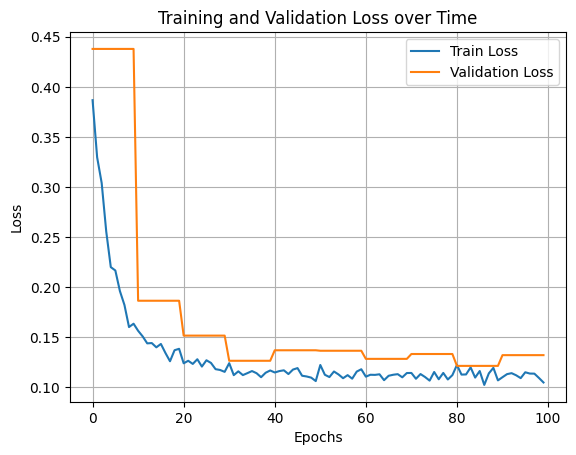
\includegraphics[width=0.48\textwidth]{figs/loss_curve.png}
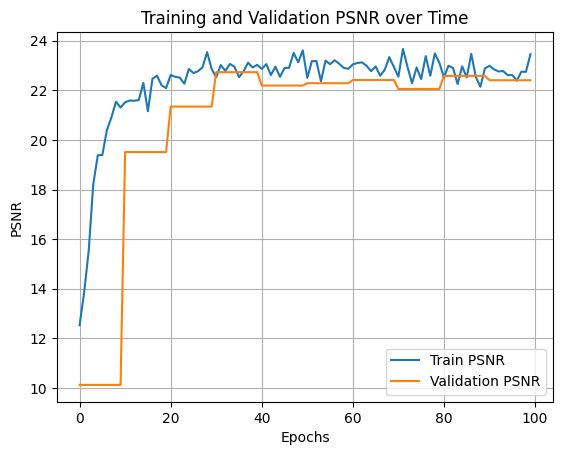
\includegraphics[width=0.48\textwidth]{figs/psnr_curve.png}
\caption{Training/validation loss and PSNR over epochs.}
\end{figure}

\subsection{Qualitative comparison}
\begin{figure}[H]
\centering
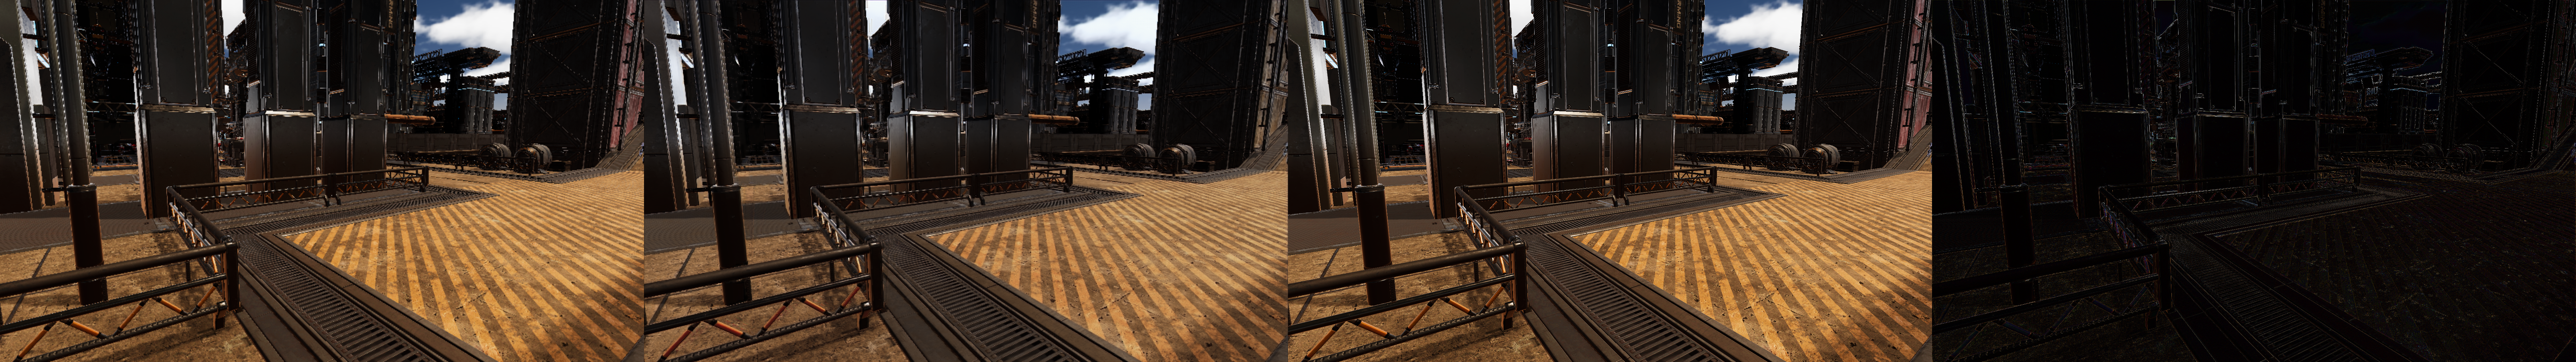
\includegraphics[width=\textwidth]{figs/qualitative_results.png}
\caption{Side by side comparison, From left to right: bicubic-upsampled input, model prediction, ground truth, and absolute difference}
\end{figure}

\subsection{PSNR summary}
\begin{table}[H]
\centering
\begin{tabular}{lc}
\toprule
Split & PSNR (dB) \\
\midrule
Train & 23.67 \\
Validation & 22.41 \\
\bottomrule
\end{tabular}
\caption{PSNR achieved by model on training and validation sets}
\end{table}

\section{Future work}

\begin{itemize}
    \item \textbf{Scaling up training}. The current model is only trained on a small subset of QRISP, due to limitations posed by the resource limits on Google Colab. Training the model on a larger dataset is likely to significantly improve performance
    
    \item \textbf{Fine tuning and deploying to custom environment}. Once the model is trained to satisfactory performance levels, it can be fine tuned to scenes from a particular game, and then can be compiled to GPU shaders or added to the graphics pipeline in some other way to create a live deployment of the system.
    
    \item \textbf{Comparing Architectures}. In this project we mainly took one existing work and tried to replicate it. Several models may be tested on the same dataset to see which performs better, and a better model may be used.
\end{itemize}

\begin{thebibliography}{9}

\bibitem{mercier2023}
A.\ Mercier, R.\ Erasmus, Y.\ Savani, M.\ Dhingra, F.\ Porikli, and G.\ Berger.
\emph{Efficient Neural Supersampling on a Novel Gaming Dataset}.
Proceedings of the IEEE/CVF International Conference on Computer Vision (ICCV), 2023, pp.\ 296--306.
\url{https://openaccess.thecvf.com/content/ICCV2023/papers/Mercier_Efficient_Neural_Supersampling_on_a_Novel_Gaming_Dataset_ICCV_2023_paper.pdf}

\bibitem{qrisp}
Qualcomm Technologies, Inc.
\emph{Qualcomm Rasterized Images Dataset (QRISP)}.
\url{https://www.qualcomm.com/developer/software/qualcomm-rasterized-images-dataset}

\end{thebibliography}

\end{document}
